\documentclass[a4paper,twoside]{article}
\usepackage[T1]{fontenc}
\usepackage[bahasa]{babel}
\usepackage{graphicx}
\usepackage{graphics}
\usepackage{listings}
\usepackage{float}
\usepackage[cm]{fullpage}
\pagestyle{myheadings}
\usepackage{etoolbox}
\usepackage{setspace} 
\usepackage{lipsum} 
\setlength{\headsep}{30pt}
\usepackage[inner=2cm,outer=2.5cm,top=2.5cm,bottom=2cm]{geometry} %margin
% \pagestyle{empty}
\lstdefinestyle{mystyle}{
    basicstyle=\footnotesize,                
   	captionpos=b,                     
   	numbers=left,                    
   	numbersep=5pt,             
   	tabsize=2
}
\lstset{style=mystyle}

\makeatletter
\renewcommand{\@maketitle} {\begin{center} {\LARGE \textbf{ \textsc{\@title}} \par} \bigskip {\large \textbf{\textsc{\@author}} }\end{center} }
\renewcommand{\thispagestyle}[1]{}
\markright{\textbf{\textsc{Laporan Perkembangan Pengerjaan Skripsi\textemdash Sem. Ganjil 2017/2018}}}

\onehalfspacing
 
\begin{document}

\title{\@judultopik}
\author{\nama \textendash \@npm} 

%ISILAH DATA DATA BERIKUT INI:
\newcommand{\nama}{Adli Fariz Bonaputra}
\newcommand{\@npm}{2012730082}
\newcommand{\tanggal}{08/05/2018} %Tanggal pembuatan dokumen
\newcommand{\@judultopik}{Konversi Javadoc ke \LaTeX} % Judul/topik anda
\newcommand{\kodetopik}{PAN4302}
\newcommand{\jumpemb}{1} % Jumlah pembimbing, 1 atau 2
\newcommand{\pembA}{Pascal Alfadian}
\newcommand{\pembB}{-}
\newcommand{\semesterPertama}{43 - Ganjil 17/18} % semester pertama kali topik diambil, angka 1 dimulai dari sem Ganjil 96/97
\newcommand{\lamaSkripsi}{2} % Jumlah semester untuk mengerjakan skripsi s.d. dokumen ini dibuat
\newcommand{\kulPertama}{Skripsi 1} % Kuliah dimana topik ini diambil pertama kali
\newcommand{\tipePR}{C} % tipe progress report :
% A : dokumen pendukung untuk pengambilan ke-2 di Skripsi 1
% B : dokumen untuk reviewer pada presentasi dan review Skripsi 1
% C : dokumen pendukung untuk pengambilan ke-2 di Skripsi 2
\maketitle

\pagenumbering{arabic}

\section{Data Skripsi} %TIDAK PERLU MENGUBAH BAGIAN INI !!!
Pembimbing utama/tunggal: {\bf \pembA}\\
Pembimbing pendamping: {\bf \pembB}\\
Kode Topik : {\bf \kodetopik}\\
Topik ini sudah dikerjakan selama : {\bf \lamaSkripsi} semester\\
Pengambilan pertama kali topik ini pada : Semester {\bf \semesterPertama} \\
Pengambilan pertama kali topik ini di kuliah : {\bf \kulPertama} \\
Tipe Laporan : {\bf \tipePR} -
\ifdefstring{\tipePR}{A}{
			Dokumen pendukung untuk {\BF pengambilan ke-2 di Skripsi 1} }
		{
		\ifdefstring{\tipePR}{B} {
				Dokumen untuk reviewer pada presentasi dan {\bf review Skripsi 1}}
			{	Dokumen pendukung untuk {\bf pengambilan ke-2 di Skripsi 2}}
		}

\section{Detail Perkembangan Pengerjaan Skripsi}
Detail bagian pekerjaan skripsi sesuai dengan rencan kerja/laporan perkembangan terkahir :
	\begin{enumerate}
		\item Melakukan studi literatur mengenai {\it syntax} \LaTeX\ dan Javadoc Doclet API.\\
		{\bf status :} Ada sejak rencana kerja skripsi.\\
		{\bf hasil :} 
		\begin{enumerate}
			\item \textbf{Javadoc}\\
			{\it Javadoc} adalah sebuah {\it tools} yang dimiliki oleh {\it Java} yang berguna untuk mengekstrak informasi dari sekumpulan {\it source file java} menjadi sebuah dokumentasi. Umumnya {\it Javadoc} menghasilkan sekumpulan {\it file} HTML yang mendeskripsikan sebuah kelas, {\it interface}, {\it method} dan {\it custom tag}. {\it Javadoc} dapat mengekstraksi informasi tersebut dari sebuah {\it package java}, sebuah {\it file java} atau keduanya.\\

\textbf{\textit{Processing of source files}}\\
{\it Javadoc} akan memproses {\it file} yang memiliki akhiran {\it ".java"} dan keseluruhan {\it file} yang terdapat di dalam folder yang sama. {\it Javadoc} dapat mengambil informasi dari 1 atau lebih {\it file java} dan sebuah {\it package}.

{\it Javadoc} dapat memproses sebuah {\it link} secara otomatis yang mengarah kepada sebuah {\it package}, kelas dan sebuah nama yang akan didokumentasikan pada saat {\it Javadoc} memprosesnya. {\it Link-link} tersebut berada pada beberapa posisi seperti:
\begin{enumerate}
	\item {\it Declaration} ({\it return types}, {\it argument types}, {\it field types}).
	\item Bagian {\it "See Also"} yang dihasilkan oleh {\it tag @see}.
	\item {\it In-line text} yang dihasilkan oleh {\it tag {@link}}.
	\item {\it Exeption} yang dihasilkan oleh {\it tag @throws}.
	\item {\it Link "Specified by"} untuk {\it member} dari sebuah {\it interface}.
	\item {\it Link "Override"} untuk {\it member} dari sebuah kelas.
	\item Ringkasan daftar tabel {\it package}, kelas dan seluruh anggota dari kelas.
	\item Turunan dari setiap {\it package} dan kelas.
	\item Indeks
\end{enumerate}

Dalam mengekstrak informasi yang terdapat dalam sebuah {\it package java} atau beberapa {\it file java} umumnya menghasilkan sebuah dokumentasi standar yang berbentuk {\it file} HTML dan format penulisan yang mengikuti standar {\it Javadoc}, akan tetapi untuk menghasilkan sebuah format dokumentasi yang diingin, dapat menggunakan sebuah {\it doclet} yang disediakan oleh {\it Javadoc}.\\

\textbf{Terminologi}\\
Terdapat beberapa istilah yang memiliki arti spesifik dalam konteks {\it Javadoc} sebagai berikut:
\begin{itemize}
	\item {\it Generated Document}\\
	Dokumen yang dihasilkan oleh {\it Javadoc tools} adalah sebuah {\it file} HTML dan dibuat oleh {\it standard doclet}
	\item {\it Name}\\
	Nama dari sebuah perangkat lunak dituliskan dalam bahasa {\it Java}. Nama-nama tersebut yaitu nama {\it package}, kelas, {\it interface}, {\it field}, {\it constructor} atau {\it method}. Nama tersebut dapat berupa informasi lengkapnya seperti {\it java.lang.String.equals(java.lang.Object)} atau informasi pendeknya seperti {\it equals(Object)}
	\item {\it Documented Classes}\\
	Detail dari sebuah kelas dan {\it interface} akan didokumentasikan pada saat {\it Javadoc} berjalan. Untuk dapat didokumentasikan, {\it source file} harus tersedia, kemudian nama dari {\it source file} atau nama dari {\it package} tersebut harus diletakkan pada {\it Javadoc command-line}
	\item {\it Included Classes}\\
	kelas dan {\it Interface} akan didokumentasikan pada saat {\it Javadoc} berjalan, hal ini sama seperti {\it Documented Classes}
	\item {\it Excluded Classes}\\
	kelas dan {\it Interface} tidak akan didokumenasikan pada saat {\it Javadoc} berjalan.
	\item {\it Referenced Classes}\\
	kelas dan {\it Interface} yang secara eksplisit disebut oleh kelas dan {\it interface} lainnya, seperti {\it return type}, {\it parameter type}, {\it cast type}, {\it extended class}, {\it implemented interface}, {\it imported class}, kelas yang digunakan pada {\it method body}, {\it @see}, {\it {@link}}, {\it {@linkplain}} dan {\it {@inheritDoc} tag} 
	\item {\it External Referenced Classes}\\
	kelas yang tidak dihasilkan saat {\it Javadoc} berjalan. Dengan kata lain, kelas tersebut tidak diletakkan pada {\it Javadoc command-line}. {\it Links} akan dihasilkan jika sebuah kelas mengatakan memiliki {\it external references} atau {\it external link}.
\end{itemize}

\textbf{\textit{Source Files}}\\
{\it Javadoc} akan menghasilkan {\it output} yang berasal dari beberapa tipe {\it file}, yaitu sebagai berikut:
\begin{itemize}
	\item {\it Class Source Code Files}\\
	Setiap kelas atau {\it interface} dapat memiliki dokumentasinya masing-masing yang terdapat pada {\it file java}
	\item {\it Package Comment Files}\\
	Setiap {\it package} dapat memiliki dokumentasinya masing-masing yang terdapat pada {\it root} folder kemudian {\it Javadoc} akan menggabungkan {\it file-file} yang terdapat pada {\it root} menjadi sebuah ringkasan. Untuk membuat dokumentasi tersebut, terdapat 2 pilihan yaitu sebuah {\it file} package.html \ref{package} atau sebuah {\it file} package-info.java \ref{package-info}.
	\begin{lstlisting}[language=Html, caption={\it File} package.html, label={package}]
	<html>
	<body>
	Provides the classes necessary to create an applet and the classes
	an applet uses to communicate with its applet context.
	
	@since 1.0
	@see java.awt
	</body>
	</html>
	\end{lstlisting}
	
	\begin{lstlisting}[language=Java, caption={\it File} package-info.java, label={package-info}]
	/**
	 * Provides the classes necessary to create an applet
	 * and the classes an applet uses to communicate
	 * with its applet context.
	 *
	 * @since 1.0
	 * @see java.awt
	 */
	 package java.lang.applet;
	\end{lstlisting}
	Ketika {\it Javadoc} memproses {\it package} tersebut, {\it Javadoc} akan melakukan beberapa langkah yaitu sebagai berikut:
	\begin{enumerate}
		\item Menyalin informasi untuk diproses. Jika {\it file} berupa HTML maka pada bagian {\it <body>} hingga {\it </body>} akan disalin.
		\item Memproses semua {\it tag} pada {\it package} yang ada.
		\item Memasukan teks yang sudah diproses tersebut pada bagian bawah halaman dokumentasi yang dihasilkan.
		\item Salin kalimat pertama pada {\it package} tersebut pada bagian atas halaman dokumentasi
	\end{enumerate}
	\item {\it Overview Comment Files}\\
	Setiap aplikasi atau sekumpulan {\it package} yang akan didokumentasikan akan memiliki dokumentasi {\it overview}. Dokumentasi tersebut dapat dibuat lebih dari 1, jika pada saat pembuatan perangkat lunak menggunakan sekumpulan {\it package} yang berbeda. Untuk membuat sebuah dokumentasi ini, perlu membuat sebuah {\it file} HTML yang umumnya bernama {\it overview.html}. Kemudian {\it Javadoc} akan memproses seperti pada {\it Package Comment Files}
	\item {\it Miscellaneous Unprocessed Files}\\
	{\it File} tersebut dapat berubah sebuah {\it graphic files}, {\it file java} dan sebuah {\it file} HTML.
\end{itemize}

\textbf{\textit{Generated Files}}\\
Secara {\it default}, {\it Javadoc} akan menggunakan {\it standard doclet} yang akan menghasilkan sebuah dokumentasi berformat HTML. Doclet tersebu akan menghasilkan {\it file} HTML secara terpisah. Terdapat 3 grup yang masing-masing grup memiliki kriterianya sendiri, 3 grup tersebut adalah sebagai berikut:
\begin{itemize}
	\item {\it Basic Content Pages}
	\begin{itemize}
		\item sebuah halaman kelas atau {\it interface} ({\it classname}.html) untuk masing-masing kelas atau {\it interface} yang akan didokumentasikan
		\item sebuah halaman {\it package} ({\it package-summary.html}) untuk masing-masing {\it package} yang akan didokumentasikan
		\item sebuah halaman {\it overview} ({\it overview-summary.html}) untuk keseluruhan sekumpulan {\it package}. Halaman ini adalah halaman utama yang dihasilkan.
	\end{itemize}
	\item {\it Cross-Reference Pages}
	\begin{itemize}
		\item sebuah halaman hirarki dari kelas untuk sekumpulan dari semua {\it package} ({\it overview-tree.html})
		\item sehalaman hirarki dari kelas untuk setiap {\it package} ({\it package-tree.html})
		\item sehalaman {\it "use"} ({\it package-use.html}) yang berisikan {\it package}, {\it classes}, {\it methods}, {\it constructors} atau {\it interface}. Jika diberikan sebuah kelas bernama A, makan halaman tersebut akan berisikan {\it subclasses} dari A, {\it methods} yang memiliki {\it return} A dan {\it methods} atau {\it constructors} dengan parameter bertipe A.
		\item sebuah halaman {\it deprecated API} ({\it deprecated-list.html}). Halaman ini adalah halaman dari sekumpulan nama yang tidak direkomendasikan untuk digunakan.
		\item sebuah halaman sekumpulan nilai {\it constant} ({\it constant-values.html}) untuk sekumpulan nilai {\it static}.
		\item sebuah halaman {\it serialized form} ({\it serialized-form.html})
		\item sebuah halaman {\it index} ({\it index-*.html}).
	\end{itemize}
	\item {\it Support Files}
	\begin{itemize}
		\item sebuah halaman bantuan ({\it help-doc.html}).
		\item sebuah halaman {\it index} ({\it index.html}) yang membuat sebuah HTML {\it frames}.
		\item beberapa {\it frame file} ({\it *-frame.html}) yang berisi sekumpulan {\it packages}, kelas dan {\it interface} dan digunakan pada saat HTML {\it frames} ditampilkan
		\item sebuah {\it file} teks {\it package list} ({\it package-list}).
		\item sebuah {\it style sheet file} ({\it stylesheet.css}) untuk mengontrol warna, jenis {\it font}, ukuran {\it font} dan posisi dari halamanan yang dihasilkan
		\item sebuah {\it doc-files} yang berisikan gambar dan beberapa contoh {\it file java}
	\end{itemize}
\end{itemize}
{\it Javadoc} akan menghasilkan 2 atau 3 HTML {\it frame}. {\it Javadoc} akan membuat minimum {\it frame} yang dibutuhkan. Jika hanya terdapat 1 {\it package}, maka {\it Javadoc} akan membuat 1 {\it frame} yang berisi dari sekumpulan kelas pada {\it package} tersebut. Jika terdapat lebih dari 2 {\it package}, maka {\it Javadoc} akan membuat 3 {\it frame} dari sekumpulan {\it package}. Jika kelas yang digunakan adalah {\it java.applet.Applet} dan semua dokumentasi yang dihasilkan akan berada pada folder yang bernama {\it apidocs}, struktur {\it file} yang dihasilkan adalah sebagai berikut:
\begin{lstlisting}[caption=Struktur {\it file} yang dihasilkan]
	apidocs						  			  		    Top directory
		index.html											  Initial page that sets up HTML frames
	* overview-summary.html 					  Lists all packages with first sentences summaries
		overview-tree.html							  Lists class hierarchy for all packages
		deprecated-list.html              Lists deprecated API for all packages
   		constant-values.html            Lists values of static fields for all packages
   		serialized-form.html            Lists serialized form for all packages
   * overview-frame.html              Lists all packages, used in upper-left frame
   		allclasses-frame.html           Lists all classes for all packages, used in
   																		lower-left frame
   		help-doc.html                   Lists user help for how these pages are organized
   		index-all.html                  Default index created without -splitindex option
   		index-files                     Directory created with -splitindex option
       		index-<number>.html         Index files created with -splitindex option
   		package-list                    Lists package names, used only for 
   																		resolving external refs
   		stylesheet.css                  HTML style sheet for defining fonts, colors and
   																		positions
   		java                            Package directory
       		applet                      Subpackage directory
            	Applet.html             Page for Applet class
            	AppletContext.html      Page for AppletContext interface
            	AppletStub.html         Page for AppletStub interface
            	AudioClip.html          Page for AudioClip interface
          * package-summary.html    	Lists classes with first sentence summaries
          														for this package
          * package-frame.html      	Lists classes in this package, used in
          														lower left-hand frame
          * package-tree.html       	Lists class hierarchy for this package
            package-use             	Lists where this package is used
            	doc-files               Directory holding image and example files
            	class-use               Directory holding pages API is used
                	Applet.html         Page for uses of Applet class
                	AppletContext.html  Page for uses of AppletContext interface
                	AppletStub.html     Page for uses of AppletStub interface
                	AudioClip.html      Page for uses of AudioClip interface
   		src-html                        Source code directory
       		java                        Package directory
           		applet                  Subpackage directory
                	Applet.html         Page for Applet source code
                	AppletContext.html  Page for AppletContext source code
                	AppletStub.html     Page for AppletStub source code
                	AudioClip.html      Page for AudioClip source code
\end{lstlisting}
		\item \textbf{Doclet}\\
		{\it Doclet} yang terdapat pada {\it Javadoc} dapat digunakan untuk menghasilkan sebuah {\it output Javadoc} yang dapat disesuaikan. Standar {\it doclet} yang dihasilkan oleh {\it Javadoc} adalah dokumentasi dengan format HTML. Selain menghasilkan {\it output} yang dapat disesuaikan, Doclet juga dapat mengekstrak informasi secara spesifik~\cite{doclet:02:doclet}.\\

\textbf{\textit{Interface-interface} pada Doclet}\\
Berikut adalah beberapa {\it interface} yang terdapat pada {\it Doclet}:
\begin{itemize}
	\item {\verb RootDoc }
	sebuah {\it interface} yang menyatakan sebuah {\it root} dari perangkat lunak yang dibuat. Dari {\it root} tersebut semua informasi dapat diekstrak. {\it Method-method} yang digunakan adalah sebagai berikut
	\begin{itemize}
		\item {\verb classes() }\\
		{\it Method} ini akan mengembalikan sejumlah kelas dan {\it interface} pada {\it package}
	\end{itemize}
	\item {\verb ClassDoc }
	sebuah {\it interface} yang menyatakan informasi dari sebuah kelas. Informasi tersebut dapat berupa nama kelas, nama {\it method} dan {\it tag}. {\it Method-method} yang digunakan adalah sebagai berikut
	\begin{itemize}
		\item {\verb name() }\\
		{\it Method} ini akan mengembalikan sebuah nama kelas atau {\it interface} pada {\it package}
		\item {\verb commentText() }\\
		{\it Method} ini akan mengembalikan sebuah informasi dari deskripsi kelas
		\item {\verb methods() }\\
		{\it Method} ini akan mengembalikan sebuah {\it array of methods}
	\end{itemize}
	\item {\verb MethodDoc }
	sebuah {\it interface} yang menyatakan informasi dari sebuah {\it method}. {\it Method-method} yang digunakan adalah sebagai berikut
	\begin{itemize}
		\item {\verb name() }\\
		{\it Method} ini akan mengembalikan sebuah nama {\it method}
		\item {\verb modifiers() }\\
		{\it Method} ini akan mengembalikan sebuah {\it access modifier} dari sebuah {\it method}
		\item {\verb returnType() }\\
		{\it Method} ini akan mengembalikan sebuah {\it return type} dari sebuah {\it method}
		\item {\verb flatSignature() }\\
		{\it Method} ini akan mengembalikan {\it signature} dari sebuah {\it method}. Jika terdapat {\it Method} dengan parameter (String x, int y), maka akan mengembalikan (String, int)
	\end{itemize}
	\item {\verb ParamTag }
	sebuah {\it interface} yang menyatakan informasi dari sebuah {\it Tag} parameter. {\it Method-method} yang digunakan adalah sebagai berikut
	\begin{itemize}
		\item {\verb name() }\\
		{\it Method} ini akan mengembalikan sebuah {\it tag @param} 
		\item {\verb parameterName() }\\
		{\it Method} ini akan mengembalikan sebuah nama parameter dari sebuah {\it method}
		\item {\verb parameterComment() }\\
		{\it Method} ini akan mengembalikan sebuah deskripsi dari parameter yang terdapat pada {\it method}
	\end{itemize}
\end{itemize}

\textbf{Penggunaan Doclet}\\
Doclet dapat menghasilkan sebuah {\it output Javadoc} yang dapat disesuaikan. Penggunaan {\it Doclet} API dapat mengekstrak bermacam-macam informasi seperti nama kelas, nama {\it method}, deskripsi singkat untuk sebuah parameter dari sebuah {\it method} hingga {\it return type} dari {\it method}.

Berikut adalah langkah-langkah untuk menggunakan {\it doclet}:
\begin{enumerate}
	\item Membuat sebuah kelas pada {\it java} sebagai {\it doclet}. {\it class java} tersebut harus meng-{\it import}  \verb com.sun.javadoc.*  untuk menggunakan {\it doclet} API.
	\item {\it Doclet} tersebut diawali dengan sebuah {\it method} \verb public  \verb static  \verb boolean  \verb start  yang memiliki parameter \verb RootDoc .
	\item {\it Compile doclet} tersebut dengan menggunakan {\it compiler} Java 2 SDK yaitu {\it javac} pada {\it command prompt(Windows)}/{\it terminal(Linux)}.
	\item Jalankan {\it Javadoc} menggunakan \verb -doclet  {\it \textbf{startingclass}} {\it option} untuk menghasilkan {\it output} yang telah disesuaikan, dimana {\it \textbf{startingclass}} adalah sebuah kelas yang sudah dibuat pada langkah 1.
\end{enumerate}

{\it File doclet} API terdapat pada direktori {\it folder jdk} yang ter-{\it install} pada komputer pada {\it subfolder}  \verb lib\tools.jar .{\it doclet} yang sudah dibuat harus di-{\it compile} menggunakan {\it file}  \verb tools.jar  dan menambahkan {\it option}  \verb -classpath  setelah {\it command}  \verb javac . Jika tidak menggunakan {\it option}  \verb -doclet  , {\it Javadoc} akan menghasilkan {\it output} standar yaitu berupa {\it file} HTML.

{\it Package}  \verb com.sun.javadoc  terdiri {\it interface} yang mendefinisikan {\it doclet} API dan sedangkan {\it file}  \verb tools.jar  berisikan {\it interface-interface} tersebut dan juga berisikan {\it private package} dengan {\it class-class} yang mengimplementasi {\it interface} tersebut serta {\it file} tools.jar berisikan pula {\it class-class} yang mengimplementasi sebuah standar {\it doclet}.

\begin{lstlisting}[language=Java, caption=kelas ListClass.java, label={program-doclet}]
	import com.sun.javadoc.*;

	public class ListClass {
		public static boolean start(RootDoc doc) {
			ClassDoc[] classes = doc.classes();
			for(int i=0, i < classes.length; i++) {
				System.out.println(classes[i]);
			}
			return true;
		}
	}
\end{lstlisting}
Potongan {\it program} ini \ref{program-doclet} adalah sebuah {\it doclet} sederhana untuk menampilkan nama-nama kelas pada {\it file java}. Hal pertama yang harus dilakukan adalah meng-{\it import package}  \verb com.sun.javadoc.* , kemudian membuat sebuah {\it method} \verb public  \verb static  \verb boolean  \verb start  dengan parameter sebuah  \verb RootDoc  doc  yang akan menampung sekumpulan {\it file java} yang akan diproses.  \verb ClassDoc  pada {\it method} tersebut akan menampung nama-nama kelas yang terdapat pada variabel  \verb doc  dengan menggunakan {\it method}  \verb classes() .
		\end{enumerate}
		
		\item Melakukan survei mengenai format penulisan pada dokumen \LaTeX\\\
		{\bf status :} Ada sejak rencana kerja skripsi.\\
		{\bf hasil :} Survei yang dilakukan adalah mengamati bab 4 dari Skripsi mahasiswa Teknik Informatika angkatan 2012 bernama Herfan Heryandi. Penulisan pada bab 4 tersebut menjadikan contoh untuk membuat struktur \LaTeX\ yang dibuat.
		
		\item Menganalisis kebutuhan perangkat lunak\\
		{\bf status :} Ada sejak rencana kerja skripsi.\\
		{\bf hasil :} 
		\begin{enumerate}
			\item \textbf{Analisis Kebutuhan Perangkat Lunak}
\label{sec:analisis}

Struktur \LaTeX\ yang digunakan memiliki format sebagai berikut.
\begin{lstlisting}[caption=Potongan kode \LaTeX, label={kode-latex}]
	\begin{enumerate}
	\item \texttt{namaKelas}\\
	{penjelasan kelas}
	
	Atribut yang dimiliki kelas ini adalah sebagai berikut.
	\begin{itemize}
		\item \texttt{atribut} -
		{penjelasan tentang atribut}.
	\end{itemize}
	
	\textit{Method} yang terdapat pada kelas Pertambahan adalah sebagai berikut.
	\begin{itemize}
		\item \texttt{method}\\
		{penjelasan method}
		
		\textbf{Parameter:}
		\begin{itemize}
			\item \texttt{parameter} - 
			{penjelasan dari parameter}.
		\end{itemize}
		
		\textbf{Return Value:} {penjelasan return-type method}\\
		\textbf{Exception:} {penjelasan exception jika terdapat exception}
		\textbf{See Also:} {penjelasan tag @see jika terdapat tag tersebut}
		\textbf{Override:} {penjelasan apabila jika terdapat {\it override method} }
	\end{itemize}

\end{lstlisting}

Potongan kode yang terdapat pada listing \ref{kode-latex} adalah struktur lengkap \LaTeX\ yang digunakan, akan dijelaskan sebagai berikut.

\begin{enumerate}
	\item {\it List level} pertama\\
	Pada {\it list level} pertama ini menampilkan sebuah nama kelas dan penjelasan terkait dengan kelas tersebut. {\it List} yang dibuat menggunakan {\it ordered list} dengan {\it command} \texttt{\string\begin\{enumerate\}}\dots\\\texttt{\string\end\{enumerate\}} dan {\it command} \texttt{\string\texttt\{namaKelas\}} akan digunakan untuk menampilkan nama kelas.
	\item {\it List level} kedua\\
	Pada {\it list level} kedua ini terdapat dua {\it list} yang masing-masing menampilkan atribut dan {\it method} yang dimiliki oleh kelas tersebut. {\it List} pertama yang dibuat menggunakan {\it unordered list} dengan {\it command} \texttt{\string\begin\{itemize\}}\dots\texttt{\string\end\{itemize\}} untuk mengisi atribut-atribut yang terdapat pada kelas ini jika kelas ini tidak memiliki atribut maka menampilkan tulisan tidak memiliki atribut. {\it Command} \texttt{\string\texttt\{atribut\}} digunakan untuk menampilkan atribut. Atribut ini menampilkan tipe atribut dan nama atribut.
	
	{\it List} kedua menggunakan {\it unordered list} dengan {\it command} \texttt{\string\begin\{itemize\}}\dots\texttt{\string\end\{itemize\}} untuk mengisi {\it method-method} yang terdapat pada kelas ini dan penjelasan terkait dengan {\it method} tersebut. {\it Command} \texttt{\string\texttt\{method\}} digunakan untuk menampilkan {\it method}. {\it Method} ini menampilkan {\it access modifier} dari {\it method}, tipe kembalian {\it method}, nama {\it method} dan daftar nama parameter.
	\item {\it List level} ketiga\\
	Pada {\it list level} ketiga ini menampilkan parameter yang digunakan pada {\it method} dan penjelasan terkait dengan parameter tersebut. {\it List} yang dibuat menggunakan {\it unordered list} dengan {\it command} \texttt{\string\begin\{itemize\}}\dots\texttt{\string\end\{itemize\}} jika {\it method} tidak memiliki parameter maka menampilkan tulisan tidak memiliki parameter dan {\it command} \texttt{\string\texttt\{parameter\}} akan digunakan untuk menampilkan parameter. Parameter ini menampilkan tipe parameter dan nama parameter.
	\item {\it Return Value} \& {\it Exception}\\
	{\it Return value} yang terdapat dalam {\it method} tersebut akan ditampilkan setelah {\it list level} ketiga jika tipe {\it return value} adalah {\verb void } maka akan menampilkan tulisan tidak memiliki {\it return value}. {\it Exception} maka ditampilkan setelah {\it Return value} jika {\it method} tidak terdapat {\it exception} maka akan menampilkan tulisan tidak memiliki {\it exception}.
	\item {\it Optional Tags}\\
	{\it Optional tags} akan menampilkan informasi dari sebuah {\it tag} \texttt{@see} atapun {\it tag} \texttt{\{@link\}}. Jika tidak ada informasi dari {\it tag - tag} tersebut akan menampilkan tulisan tidak ada.
	\item {\it Override}\\
	{\it Override} akan menampilkan informasi apakah {\it method} dari sebuah {\it superclass} ditulis kembali di sebuah {\it subclass}. jika tidak ada informasi tersebut maka bagian penjelasan akan dihilangkan.
\end{enumerate}

Perangkat lunak yang dibuat akan menerima sebuah masukan berupa sekumpulan {\it file java} yang berada di dalam sebuah {\it package}. Struktur kode {\it java} yang digunakan memiliki format sebagai berikut.

\begin{lstlisting}[language=Java, caption=Contoh kode {\it java} dari {\it superclass} yang diuji, label={kode-java-superclass}]
package javadoc;

/**
 * Kelas Abstract OperasiMatematika
 * @author Adli Fariz Bonaputra
 */
public abstract class OperasiMatematikaInterface {
  
  /**
   * Method untuk menghasilkan perhitungan 2 buah bilangan
   * @param a Bilangan pertama
   * @param b Bilagan kedua
   * @return hasil perhitungan 2 buah bilangan
   */
  public int calculate(int a, int b){return 0;}
}
\end{lstlisting}

\begin{lstlisting}[language=Java, caption=Contoh kode {\it java} dari {\it subclass} yang diuji, label={kode-java-subclass}]
package javadoc;

/**
 * Kelas ini merupakan Kelas Pertambahan kelas ini memiliki beberapa fungsi
 * yaitu {@link #calculate(int,int) calculate}
 *
 * @author Adli Fariz Bonaputra
 * @see "Pertambahan"
 *
 */
public class Pertambahan extends OperasiMatematikaInterface {

  /**
   * Atribut A
   */
  private int a;
  /**
   * Atribut B
   */
  private int b;

  @Override
  public int calculate(int a, int b) {
    int hasil = 0;
    hasil = a + b + 10;
    return hasil;
  }
}
\end{lstlisting}

Potongan kode yang terdapat pada listing \ref{kode-java-superclass} dan \ref{kode-java-subclass} adalah struktur {\it file java} yang digunakan, akan dijelaskan sebagai berikut.

\begin{enumerate}
	\item Setiap {\it file java} harus terletak di dalam sebuah {\it package} yang sama.
	\item Setiap deklarasi kelas harus diawali dengan huruf kapital serta memiliki javadoc untuk penjelasan tentang kelas tersebut dan secara opsional dapat menambahkan {\it tag - tag} javadoc seperti {\it tag} \texttt{@see} sebagai penunjuk ke sebuah referensi dan {\it tag} \texttt{\{@link\}} sebagai penunjuk ke dokumentasi sebuah {\it package}, {\it class} ataupun {\it method} yang dimiliki oleh kelas lain.
	\item Setiap deklarasi atribut harus memiliki {\it access modifier}, tipe atribut dan nama atribut serta memiliki javadoc untuk penjelasan tentang atribut tersebut.
	\item Seiap deklarasi {\it method} harus memiliki {\it access modifier}, tipe kembalian, nama {\it method}, tipe dan variabel parameter serta memiliki javadoc untuk penjelasan {\it method}, parameter yang digunakan dan hasil kembalian sebuah {\it method}.
\end{enumerate}

%{\it Package} yang berisikan sekumpulan {\it file java} tersebut akan menjadi sebuah masukan perangkat lunak dan akan menghasilkan sebuah dokumen dalam format \LaTeX.
Hasil dari sebuah perangkat lunak yang dibuat adalah sebuah {\it file} berformat \LaTeX. Perangkat lunak akan membaca satu persatu {\it file java} dan informasi yang terdapat pada setiap {\it file java} tersebut dimasukan ke dalam {\it file} \LaTeX.

\begin{lstlisting}[caption=Contoh hasil konversi {\it Javadoc} ke \LaTeX, label={hasil}]
\begin{enumerate}
	\item \texttt{Pertambahan}\\
	Kelas ini merupakan Kelas Pertambahan.
	
	Atribut yang dimiliki kelas ini adalah sebagai berikut.
	\begin{itemize}
		\item \texttt{int a} -
		Atribut A.
		\item \texttt{int b} -
		Atribut B.
	\end{itemize}
	
	\textit{Method} yang terdapat pada kelas Pertambahan adalah sebagai berikut.
	\begin{itemize}
		\item \texttt{public int pertambahan(int a, int b)}\\
		Method Pertambahan.
		
		\textbf{Parameter:}
		\begin{itemize}
			\item \texttt{int a} - 
			Bilangan Pertama.
			\item \texttt{int b} - 
			Bilangan Kedua.
		\end{itemize}
		
		\textbf{Return Value:} hasil penjumlahan 2 buah bilangan.\\
		\textbf{Exception:} tidak memiliki \textit{exception}.
		\textbf{Override:} \textt{pertambahan} dari kelas \textt{operasiMatematikaInterface}
	\end{itemize}
\end{enumerate}
\end{lstlisting}

Hasil konversi \ref{hasil} akan menampilkan nama kelas serta penjelasan kelas tersebut, atribut yang digunakan serta penjelasan untuk setiap atributnya, {\it method} yang digunakan serta penjelasan {\it method}, parameter yang digunakan serta penjelasan setiap parameternya, {\it return value} dan {\it exception}.

\textbf{Analisis Program Sejenis TeXDoclet}
\label{sec:texdoclet}
TeXDoclet merupakan sebuah program yang mengimplementasi {\it Doclet} yang dimiliki oleh {\it Java}. Program ini akan mengkonversi sekumpulan {\it file java} yang terletak di dalam satu {\it package} yang sama. TeXDoclet dapat menghasilkan dokumen berupa {\it file} \LaTeX\ atau {\it file} PDF. Untuk dapat menghasilkan {\it file} PDF, TeXDoclet mengintegrasikan Lua\LaTeX\ untuk menghasilkan dokumen PDF dari sebuah {\it file} \LaTeX.

TeXDoclet memiliki beberapa {\it option} yang dapat digunakan, akan dijelaskan sebagai berikut.
\begin{enumerate}
	\item \texttt{-sectionlevel <level>}\\
	Untuk menentukan {\it level} teratas dari {\it section} sebuah dokumen. {\it Section} tersebut bisa berupa {\it chapter}, {\it section} atau {\it subsection}
	\item \texttt{-createPdf}\\
	Untuk menghasilkan {\it file} PDF dari sebuah hasil {\it file} \LaTeX\ dengan menggunakan Lua\LaTeX.
	\item \texttt{-twosided}\\
	Untuk menghasilkan dokumen 2 sisi. Jika dokumen tersebut menggunakan {\it option} ini maka dokumen tersebut pada saat dicetak akan memiliki 2 sisi yaitu depan dan belakang.
	\item \texttt{-texinit <file>}\\
	Untuk menambahkan {\it command-command} yang lain sebelum {\it command} \texttt{\string\begin\{document\}}.
	\item \texttt{-docclass <class>}\\
	Untuk menentukan tipe dokumen yang akan dibuat. {\it Default} untuk {\it option} adalah tipe dokumen {\it report}.
\end{enumerate}
		\end{enumerate}

		\item Merancang perangkat lunak\\
		{\bf status :} Ada sejak rencana kerja skripsi.\\
		{\bf hasil :} 
Rancangan kelas dibawah ini akan menampilkan keseluruhan kelas yang akan digunakan. Deskripsi kelas berserta fungsi dari diagram kelas tersebut adalah sebagai berikut:

\begin{figure}[H]
	\centering  
	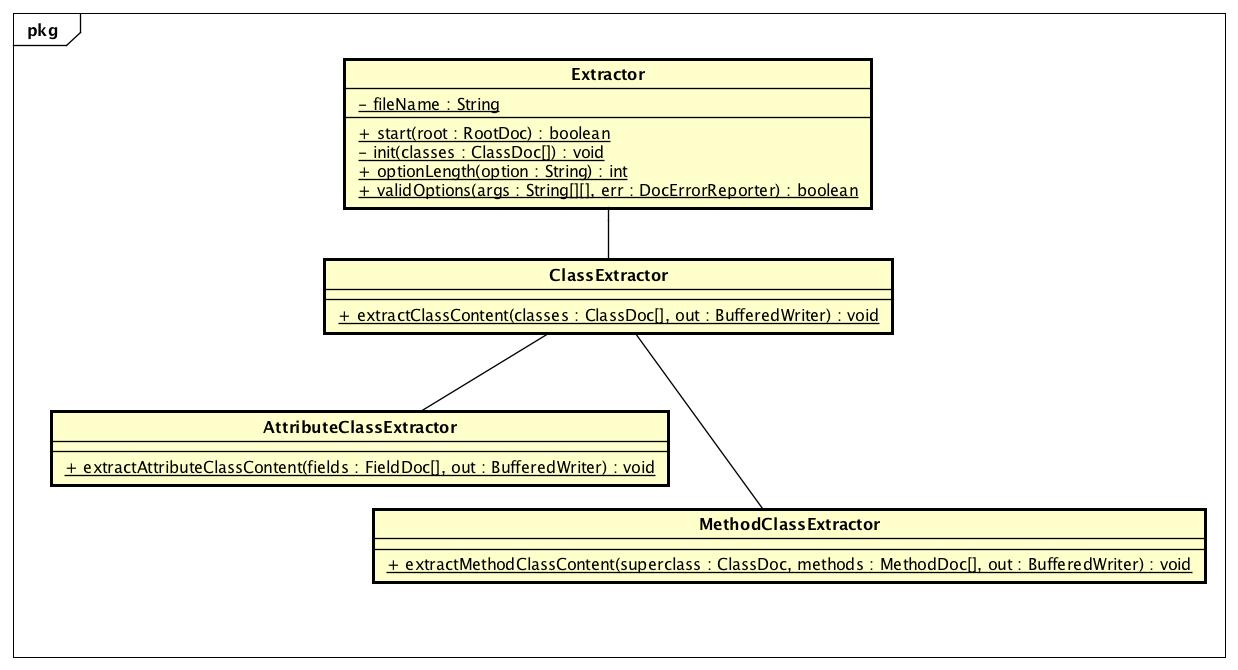
\includegraphics[scale=0.4]{Gambar/kelas-diagram}  
	\caption[Kelas Diagram]{Kelas Diagram} 
	\label{fig:kelas-diagram} 
\end{figure} 

\begin{enumerate}
\item \texttt{AttributeClassExtractor}\\ 
Kelas ini merupakan kelas untuk mengambil informasi sebuah atribut yang
 terdapat pada kelas.

Kelas ini tidak memiliki atribut. \textit{Method-method} yang dimiliki kelas ini adalah sebagai berikut.
\begin{itemize}
\item \texttt{public static void extractAttributeClassContent(com.sun.javadoc.FieldDoc[] fields, BufferedWriter out)}\\ 
\textit{Method} ini akan menampilkan atribut-atribut yang dimiliki oleh
 sebuah kelas

\textbf{Parameter:}
\begin{itemize}
\item \texttt{com.sun.javadoc.FieldDoc[] fields} - 
sebuah array berisikan sejumlah atribut dari kelas
\item \texttt{BufferedWriter out} - 
turunan dari kelas \texttt{Writer} yang digunakan untuk menulis
 file text
\end{itemize}
\textbf{Kembalian}: Tidak memiliki \textit{return value}

\textbf{Exception}: Tidak memiliki \textit{exception}

\end{itemize}
\item \texttt{ClassExtractor}\\ 
Kelas ini merupakan kelas untuk mengambil informasi dari sebuah kelas.

Kelas ini tidak memiliki atribut. \textit{Method-method} yang dimiliki kelas ini adalah sebagai berikut.
\begin{itemize}
\item \texttt{public static void extractClassContent(com.sun.javadoc.ClassDoc[] classes, BufferedWriter out)}\\ 
\textit{Method} ini akan menampilkan nama kelas berserta penjelasan dari sebuah kelas

\textbf{Parameter:}
\begin{itemize}
\item \texttt{com.sun.javadoc.ClassDoc[] classes} - 
sebuah array berisikan sejumlah kelas
\item \texttt{BufferedWriter out} - 
turunan dari kelas \texttt{Writer} yang digunakan untuk menulis file text
\end{itemize}
\textbf{Kembalian}: Tidak memiliki \textit{return value}

\textbf{Exception}: Tidak memiliki \textit{exception}

\end{itemize}
\item \texttt{Extractor}\\ 
Kelas ini merupakan kelas untuk menjalan \textit{custom doclet}.

Atribut yang dimiliki kelas ini adalah sebagai berikut.
\begin{itemize}
\item \texttt{String fileName} - atribut untuk nama \textit{file}
\end{itemize}
\textit{Method-method} yang dimiliki kelas ini adalah sebagai berikut.
\begin{itemize}
\item \texttt{public static boolean start(RootDoc root)}\\ 
\textit{Method} ini berperan sebagai \textit{method} untuk menjalankan
 \textit{custom doclet}

\textbf{Parameter:}
\begin{itemize}
\item \texttt{RootDoc root} - 
berperan sebagai mengambil seluruh informasi spesifik dari
 \textit{option} yang terdapat pada \textit{command-line} sebuah
 \textit{terminal}. Selain itu berperan juga untuk mengambil informasi dari
 sekumpulan \textit{file java} yang akan di proses.
\end{itemize}
\textbf{Kembalian}: kondisi true

\textbf{Exception}: Tidak memiliki \textit{exception}

\item \texttt{private static void init(com.sun.javadoc.ClassDoc[] classes)}\\ 
\textit{Method} ini berperan untuk menulis kedalam sebuah \textit{file}
 saat \textit{javadoc} berjalan.

\textbf{Parameter:}
\begin{itemize}
\item \texttt{com.sun.javadoc.ClassDoc[] classes} - 
sebuah array yang berisikan sekumpulan \textit{file java}
 yang akan di proses.
\end{itemize}
\textbf{Kembalian}: Tidak memiliki \textit{return value}

\textbf{Exception}: Tidak memiliki \textit{exception}

\item \texttt{public static int optionLength(String option)}\\ 
Method untuk menghitung banyak option yang digunakan pada
 \textit{command-line}

\textbf{Parameter:}
\begin{itemize}
\item \texttt{String option} - 
sebuah option
\end{itemize}
\textbf{Kembalian}: panjang setiap option

\textbf{Exception}: Tidak memiliki \textit{exception}

\item \texttt{public static boolean validOptions(java.lang.String[][] args, DocErrorReporter err)}\\ 
Pengecekan option valid

\textbf{Parameter:}
\begin{itemize}
\item \texttt{java.lang.String[][] args} - 
String array 2 dimensi dari option
\item \texttt{DocErrorReporter err} - 
sebuah error jika tidak terdapat option tersebut.
\end{itemize}
\textbf{Kembalian}: bernilai true jika option tersebut dikenali, false jika option
 tersebut tidak dikenali

\textbf{Exception}: Tidak memiliki \textit{exception}

\end{itemize}
\item \texttt{MethodClassExtractor}\\ 
Kelas ini merupakan kelas untuk mengambil informasi sebuah \textit{method}
 terdapat pada kelas.

Kelas ini tidak memiliki atribut. \textit{Method-method} yang dimiliki kelas ini adalah sebagai berikut.
\begin{itemize}
\item \texttt{public static void extractMethodClassContent(ClassDoc superclass, \\com.sun.javadoc.MethodDoc[] methods, BufferedWriter out)}\\ 
\textit{Method} ini akan menampilkan \textit{method-method} yang dimiliki
 oleh sebuah kelas

\textbf{Parameter:}
\begin{itemize}
\item \texttt{ClassDoc superclass} - 
sebuah objek ClassDoc
\item \texttt{com.sun.javadoc.MethodDoc[] methods} - 
sebuah array berisikan sejumlah \textit{method} dari kelas
\item \texttt{BufferedWriter out} - 
turunan dari kelas \texttt{Writer} yang digunakan untuk menulis
 file text
\end{itemize}
\textbf{Kembalian}: Tidak memiliki \textit{return value}

\textbf{Exception}: Tidak memiliki \textit{exception}

\end{itemize}
\end{enumerate}

\section{Rancangan Antarmuka}
\label{sec:antarmuka}
Rancangan antarmuka perangkat lunak yang dibuat adalah melalui sebuah {\it terminal} pada {\it Linux} dan {\it command prompt} pada {\it Windows}. Berikut adalah antarmuka jika menggunakan {\it terminal} pada {\it Linux}: 

\begin{figure}[H]
	\centering  
	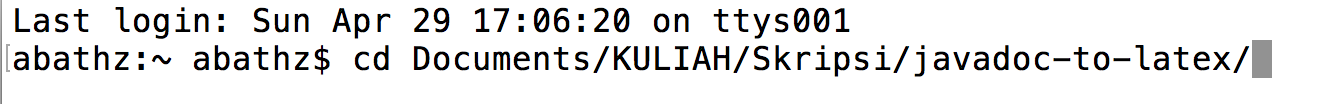
\includegraphics[scale=0.5]{Gambar/1}  
	\caption[]{Mengarahkan kedalam folder dari perangkat lunak} 
	\label{fig:1} 
\end{figure}
Langkah pertama adalah berpindah dari direktori awal ke direktori perangkat lunak yang dibuat. Untuk berpindah direktori perlukan {\it command} \texttt{cd} atau kepanjangan dari {\it change directory} lalu diikuti dengan lokasi direktori yang diinginkan. Pada gambar \ref{fig:1} direktori perangkat lunak terdapat di dalam folder Document lalu folder KULIAH lalu folder Skripsi dan terakhir folder javadoc-to-latex kemudian tekan tombol {\it enter} lalu direktori akan langsung berpindah ke direktori yang dituju.

\begin{figure}[H]
	\centering  
	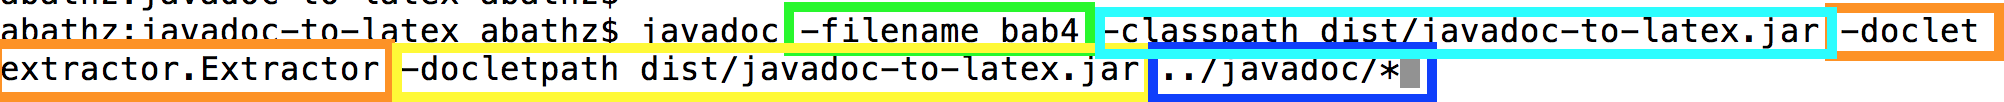
\includegraphics[scale=0.5]{Gambar/2}  
	\caption[]{Memasukkan {\it option} yang akan digunakan} 
	\label{fig:2} 
\end{figure}
Langkah kedua adalah menjalan perangkat lunak yang dibuat. Diawali dengan command \texttt{javadoc} lalu dikuti 5 buah argumen. Argumen pertama(hijau) adalah {\it option} untuk menamai {\it file} sesuai dengan yang ditentukan. Sebagai contoh pada gambar \ref{fig:2}, {\it file} akan bernama "bab4", jika argumen pertama tidak dimasukkan pada {\it command-line} maka nama dari {\it file} tersebut secara otomatis menjadi "doc". Argumen kedua(biru muda) berperan sebagai penunjuk kelas-kelas yang digunakan. Argumen kedua ini bersifat {\it optional}, jika kode program yang akan didokumentasikan menggunakan {\it external library} maka argumen ini digunakan. Argumen ketiga(jingga) adalah sebuah kelas untuk menjalankan {\it custom doclet} dari perangkat lunak yang dibuat. Argumen ketiga tersebut akan menjalankan kelas bernama \texttt{Extractor} yang terdapat didalam {\it package} \texttt{extractor}. Kemudian argumen keempat(kuning) adalah {\it custom doclet} yang berperan untuk mengambil informasi kelas, atribut, {\it method} dari sekumpulan {\it file java}. Argumen kelima(biru) adalah lokasi sekumpulan {\it file java} yang akan diproses. Pada gambar \ref{fig:2}, lokasi {\it file-file} tersebut terdapat pada folder javadoc. Folder javadoc tersebut berada direktori folder Skripsi.

\begin{figure}[H]
	\centering  
	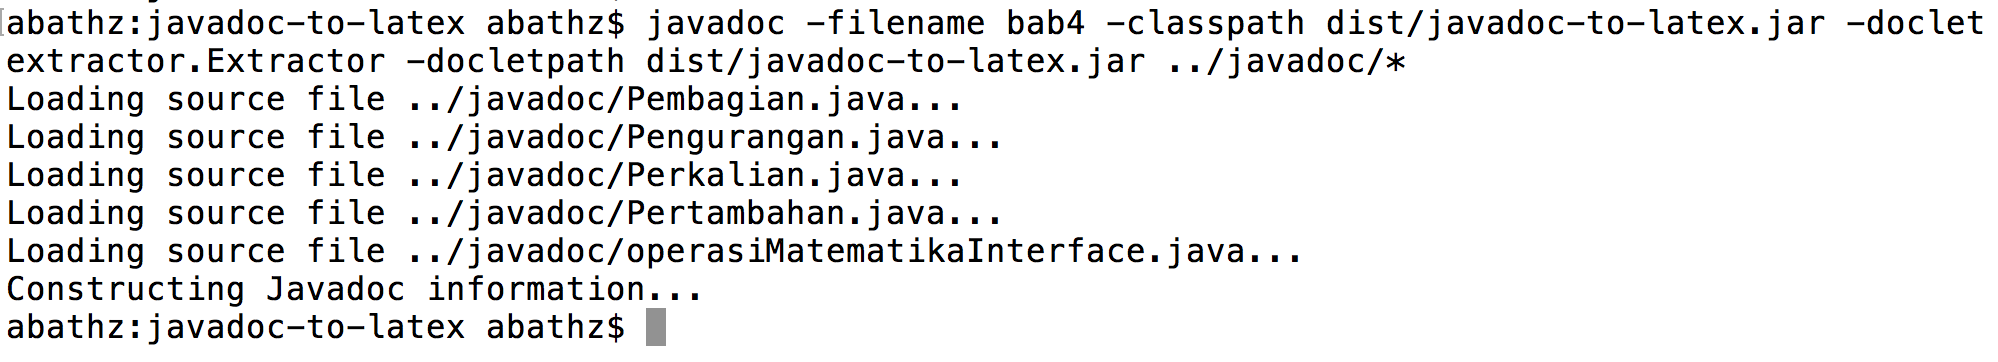
\includegraphics[scale=0.5]{Gambar/3}  
	\caption[]{Hasil tampilan jika proses konversi selesai} 
	\label{fig:3} 
\end{figure}
Perangkat lunak yang dibuat akan membaca seluruh isi folder yang dituju, pada contoh gambar \ref{fig:3}, terdapat 5 {\it file java} yang terdapat didalam folder javadoc. Lalu perangkat lunak akan melakukan ekstrasi informasi terhadap masing-masing {\it file} tersebut. Jika proses ekstraksi selesai maka proses berhenti.

		\item Mengimplementasi Javadoc Doclet API\\
		{\bf status :} Ada sejak rencana kerja skripsi.\\
		{\bf hasil :} Pada bagian ini akan dibahas mengenai implementasi perangkat lunak yang telah dibangun. Sub bab ini terdiri atas tiga bagian, yaitu lingkungan perangkat lunak, hasil implementasi perangkat lunak, dan Pengujian perangkat lunak.

\subsection{Lingkungan Perangkat Lunak}
\label{sec:lingkungan perangkat lunak}
Dalam proses membangun perangkat lunak ini digunakan spesifikasi perangkat sebagai berikut.

\begin{enumerate}
	\item Processor: Intel Core i7 2.5-3.7GHz 
	\item RAM: 16.00 GB DDR3	
	\item Harddisk : 512MB SSD
	\item VGA : Intel Iris Pro dan AMD Radeon R9 M370X
	\item Sistem Operasi: macOS High Sierra
	\item Versi Java: 1.8.0\_121
	\item Code Editor: Netbeans 8.2
\end{enumerate}

\subsection{Hasil Implementasi}
\label{sec:hasil implementasi}
Kode program pada perangkat lunak ditulis dengan bahasa pemrograman {\it java}. Perangkat lunak akan menghasilkan sebuah {\it file} \LaTeX\ yang berisikan dokumentasi sekumpulan kelas-kelas {\it java}. Berikut {\it file} \LaTeX\ yang dihasilkan dari kode program perangkat lunak yang telah dibuat.
\begin{lstlisting}[caption=Hasil Implementasi]
\begin{enumerate}
\item \texttt{AttributeClassExtractor}\\ 
Kelas ini merupakan kelas untuk mengambil informasi sebuah atribut yang
 terdapat pada kelas.

Kelas ini tidak memiliki atribut. \textit{Method-method} yang dimiliki kelas ini adalah sebagai berikut.
\begin{itemize}
\item \texttt{public static void extractAttributeClassContent(com.sun.javadoc.FieldDoc[] fields, BufferedWriter out)}\\ 
\textit{Method} ini akan menampilkan atribut-atribut yang dimiliki oleh
 sebuah kelas

\textbf{Parameter:}
\begin{itemize}
\item \texttt{com.sun.javadoc.FieldDoc[] fields} - 
sebuah array berisikan sejumlah atribut dari kelas
\item \texttt{BufferedWriter out} - 
turunan dari kelas \texttt{Writer} yang digunakan untuk menulis
 file text
\end{itemize}
\textbf{Kembalian}: Tidak memiliki \textit{return value}

\textbf{Exception}: Tidak memiliki \textit{exception}

\end{itemize}
\item \texttt{ClassExtractor}\\ 
Kelas ini merupakan kelas untuk mengambil informasi dari sebuah kelas.

Kelas ini tidak memiliki atribut. \textit{Method-method} yang dimiliki kelas ini adalah sebagai berikut.
\begin{itemize}
\item \texttt{public static void extractClassContent(com.sun.javadoc.ClassDoc[] classes, BufferedWriter out)}\\ 
\textit{Method} ini akan menampilkan nama kelas berserta penjelasan dari sebuah kelas

\textbf{Parameter:}
\begin{itemize}
\item \texttt{com.sun.javadoc.ClassDoc[] classes} - 
sebuah array berisikan sejumlah kelas
\item \texttt{BufferedWriter out} - 
turunan dari kelas \texttt{Writer} yang digunakan untuk menulis file text
\end{itemize}
\textbf{Kembalian}: Tidak memiliki \textit{return value}

\textbf{Exception}: Tidak memiliki \textit{exception}

\end{itemize}
\item \texttt{Extractor}\\ 
Kelas ini merupakan kelas untuk menjalan \textit{custom doclet}.

Atribut yang dimiliki kelas ini adalah sebagai berikut.
\begin{itemize}
\item \texttt{String fileName} - atribut untuk nama \textit{file}
\end{itemize}
\textit{Method-method} yang dimiliki kelas ini adalah sebagai berikut.
\begin{itemize}
\item \texttt{public static boolean start(RootDoc root)}\\ 
\textit{Method} ini berperan sebagai \textit{method} untuk menjalankan
 \textit{custom doclet}

\textbf{Parameter:}
\begin{itemize}
\item \texttt{RootDoc root} - 
berperan sebagai mengambil seluruh informasi spesifik dari
 \textit{option} yang terdapat pada \textit{command-line} sebuah
 \textit{terminal}. Selain itu berperan juga untuk mengambil informasi dari
 sekumpulan \textit{file java} yang akan di proses.
\end{itemize}
\textbf{Kembalian}: kondisi true

\textbf{Exception}: Tidak memiliki \textit{exception}

\item \texttt{private static void init(com.sun.javadoc.ClassDoc[] classes)}\\ 
\textit{Method} ini berperan untuk menulis kedalam sebuah \textit{file}
 saat \textit{javadoc} berjalan.

\textbf{Parameter:}
\begin{itemize}
\item \texttt{com.sun.javadoc.ClassDoc[] classes} - 
sebuah array yang berisikan sekumpulan \textit{file java}
 yang akan di proses.
\end{itemize}
\textbf{Kembalian}: Tidak memiliki \textit{return value}

\textbf{Exception}: Tidak memiliki \textit{exception}

\item \texttt{public static int optionLength(String option)}\\ 
Method untuk menghitung banyak option yang digunakan pada
 \textit{command-line}

\textbf{Parameter:}
\begin{itemize}
\item \texttt{String option} - 
sebuah option
\end{itemize}
\textbf{Kembalian}: panjang setiap option

\textbf{Exception}: Tidak memiliki \textit{exception}

\item \texttt{public static boolean validOptions(java.lang.String[][] args, DocErrorReporter err)}\\ 
Pengecekan option valid

\textbf{Parameter:}
\begin{itemize}
\item \texttt{java.lang.String[][] args} - 
String array 2 dimensi dari option
\item \texttt{DocErrorReporter err} - 
sebuah error jika tidak terdapat option tersebut.
\end{itemize}
\textbf{Kembalian}: bernilai true jika option tersebut dikenali, false jika option
 tersebut tidak dikenali

\textbf{Exception}: Tidak memiliki \textit{exception}

\end{itemize}
\item \texttt{MethodClassExtractor}\\ 
Kelas ini merupakan kelas untuk mengambil informasi sebuah \textit{method}
 terdapat pada kelas.

Kelas ini tidak memiliki atribut. \textit{Method-method} yang dimiliki kelas ini adalah sebagai berikut.
\begin{itemize}
\item \texttt{public static void extractMethodContent(ClassDoc superclass, com.sun.javadoc.MethodDoc[] methods, BufferedWriter out)}\\ 
\textit{Method} ini akan menampilkan \textit{method-method} yang dimiliki
 oleh sebuah kelas

\textbf{Parameter:}
\begin{itemize}
\item \texttt{ClassDoc superclass} - 
sebuah objek ClassDoc
\item \texttt{com.sun.javadoc.MethodDoc[] methods} - 
sebuah array berisikan sejumlah \textit{method} dari kelas
\item \texttt{BufferedWriter out} - 
turunan dari kelas \texttt{Writer} yang digunakan untuk menulis
 file text
\end{itemize}
\textbf{Kembalian}: Tidak memiliki \textit{return value}

\textbf{Exception}: Tidak memiliki \textit{exception}

\end{itemize}
\end{enumerate}

\end{lstlisting}

		\item Melakukan pengujian perangkat lunak\\
		{\bf status :} Pengujian Fungsional sudah dilakukan, Pengujian Eksperimental masih terdapat kendala \\
		{\bf hasil :} \subsection{Pengujian Fungsional}
\label{sec:pengujian fungsional}
Pada pengujian fungsional dilakukan untuk mengetahui fungsi-fungsi yang terdapat pada perangkat lunak berjalan sesuai dengan yang diharapkan. Status pengujian dibagi menjadi 2 yaitu "OK" dan "GAGAL". Berikut ini adalah hasil pengujian fungsional yang telah dilakukan.
\begin{enumerate}
	\item Langkah Pengujian: Memanggil fungsi \texttt{extractClassContent}\\
	Hal yang diharapkan: pada saat fungsi \texttt{extractClassContent} dipanggil maka informasi berkaitan dengan kelas tersebut terekstraksi.\\
	Hasil Pengujian: Informasi yang berkaitan dengan kelas telah terekstraksi.\\
	Status: OK
	\item Langkah Pengujian: Memanggil fungsi \texttt{extractAttributeClassContent}\\
	Hal yang diharapkan: pada saat fungsi \texttt{extractAttributeClassContent} dipanggil maka informasi berkaitan dengan atribut-atribut yang terdapat pada kelas tersebut terekstraksi.\\
	Hasil Pengujian: Informasi yang berkaitan dengan atribut-atribut yang terdapat pada kelas telah terekstraksi.\\
	Status: OK
	\item Langkah Pengujian: Memanggil fungsi \texttt{extractMethodClassContent}\\
	Hal yang diharapkan: pada saat fungsi \texttt{extractMethodClassContent} dipanggil maka informasi berkaitan dengan fungsi-fungsi yang terdapat pada kelas tersebut terekstraksi.\\
	Hasil Pengujian: Informasi yang berkaitan dengan fungsi-fungsi yang terdapat pada kelas telah terekstraksi.\\
	Status: OK
\end{enumerate}

\subsection{Pengujian Eksperimental}
\label{sec:pengujian eksperimental}
Pengujian eksperimental dilakukan terhadap 3 pengujian yaitu pengujian terhadap kode program sederhana, pengujian terhadap kode program perangkat lunak dan pengujian terhadap kode program yang memiliki jumlah {\it file} yang banyak.

\subsubsection{Pengujian Terhadap Kode Program Sederhana}
\label{sec:pengujian sederhana}
Pengujian pertama ini melibatkan kode program sederhana yaitu Operasi Matematika. Kode program ini memiliki 5 buah kelas yaitu \texttt{OperasiMatematikaInterface}, \texttt{Pembagian}, \texttt{Perkalian}, \texttt{Pertambahan} dan \texttt{Pengurangan}. Berikut hasil {\it file} \LaTeX\ yang dihasilkan.
\begin{lstlisting}[caption=Hasil Pengujian Pertama]
\begin{enumerate}
\item \texttt{OperasiMatematikaInterface}\\ 
Kelas Abstract OperasiMatematika.

Kelas ini tidak memiliki atribut. \textit{Method-method} yang dimiliki kelas ini adalah sebagai berikut.
\begin{itemize}
\item \texttt{public int calculate(int a, int b)}\\ 
Method untuk menghasilkan perhitungan 2 buah bilangan

\textbf{Parameter:}
\begin{itemize}
\item \texttt{int a} - 
Bilangan pertama
\item \texttt{int b} - 
Bilagan kedua
\end{itemize}
\textbf{Kembalian}: hasil perhitungan 2 buah bilangan

\textbf{Exception}: Tidak memiliki \textit{exception}

\end{itemize}
\item \texttt{Pembagian}\\ 
Kelas ini merupakan Kelas Pembagian.

Atribut yang dimiliki kelas ini adalah sebagai berikut.
\begin{itemize}
\item \texttt{int a} - Atribut A
\item \texttt{int b} - Atribut B
\end{itemize}
\textit{Method-method} yang dimiliki kelas ini adalah sebagai berikut.
\begin{itemize}
\item \texttt{public int calculate(int a, int b)}\\ 
Method untuk menghasilkan perhitungan 2 buah bilangan

\textbf{Parameter:}
\begin{itemize}
\item \texttt{int a} - 
Bilangan pertama
\item \texttt{int b} - 
Bilagan kedua
\end{itemize}
\textbf{Kembalian}: hasil perhitungan 2 buah bilangan

\textbf{Exception}: Tidak memiliki \textit{exception}

\end{itemize}
\item \texttt{Pengurangan}\\ 
Kelas ini merupakan Kelas Pengurangan.

Atribut yang dimiliki kelas ini adalah sebagai berikut.
\begin{itemize}
\item \texttt{int a} - Atribut A
\item \texttt{int b} - Atribut B
\end{itemize}
\textit{Method-method} yang dimiliki kelas ini adalah sebagai berikut.
\begin{itemize}
\item \texttt{public int calculate(int a, int b)}\\ 
Method untuk menghasilkan perhitungan 2 buah bilangan

\textbf{Parameter:}
\begin{itemize}
\item \texttt{int a} - 
Bilangan pertama
\item \texttt{int b} - 
Bilagan kedua
\end{itemize}
\textbf{Kembalian}: hasil perhitungan 2 buah bilangan

\textbf{Exception}: Tidak memiliki \textit{exception}

\end{itemize}
\item \texttt{Perkalian}\\ 
Kelas ini merupakan Kelas Perkalian.

Atribut yang dimiliki kelas ini adalah sebagai berikut.
\begin{itemize}
\item \texttt{int a} - Atribut A
\item \texttt{int b} - Atribut B
\end{itemize}
\textit{Method-method} yang dimiliki kelas ini adalah sebagai berikut.
\begin{itemize}
\item \texttt{public int calculate(int a, int b)}\\ 
Method untuk menghasilkan perhitungan 2 buah bilangan

\textbf{Parameter:}
\begin{itemize}
\item \texttt{int a} - 
Bilangan pertama
\item \texttt{int b} - 
Bilagan kedua
\end{itemize}
\textbf{Kembalian}: hasil perhitungan 2 buah bilangan

\textbf{Exception}: Tidak memiliki \textit{exception}

\end{itemize}
\item \texttt{Pertambahan}\\ 
Kelas ini merupakan Kelas Pertambahan.

Atribut yang dimiliki kelas ini adalah sebagai berikut.
\begin{itemize}
\item \texttt{int a} - Atribut A
\item \texttt{int b} - Atribut B
\end{itemize}
\textit{Method-method} yang dimiliki kelas ini adalah sebagai berikut.
\begin{itemize}
\item \texttt{public int calculate(int a, int b)}\\ 
Method untuk menghasilkan perhitungan 2 buah bilangan

\textbf{Parameter:}
\begin{itemize}
\item \texttt{int a} - 
Bilangan pertama
\item \texttt{int b} - 
Bilagan kedua
\end{itemize}
\textbf{Kembalian}: hasil perhitungan 2 buah bilangan

\textbf{Exception}: Tidak memiliki \textit{exception}

\end{itemize}
\end{enumerate}

\end{lstlisting}

\subsubsection{Pengujian Terhadap Kode Program Perangkat Lunak}
\label{sec:pengujian perangkat lunak}
Pengujian kedua ini melibatkan kode program perangkat lunak. Kode program ini memiliki 4 buah kelas yaitu \texttt{Extractor}, \texttt{ClassExtractor}, \texttt{AttributeClassExtractor} dan \texttt{MethodClassExtractor}. Berikut hasil {\it file} \LaTeX\ yang dihasilkan.

\begin{lstlisting}[caption=Hasil Pengujian Kedua]
\begin{enumerate}
\item \texttt{AttributeClassExtractor}\\ 
Kelas ini merupakan kelas untuk mengambil informasi sebuah atribut yang
 terdapat pada kelas.

Kelas ini tidak memiliki atribut. \textit{Method-method} yang dimiliki kelas ini adalah sebagai berikut.
\begin{itemize}
\item \texttt{public static void extractAttributeClassContent(com.sun.javadoc.FieldDoc[] fields, BufferedWriter out)}\\ 
\textit{Method} ini akan menampilkan atribut-atribut yang dimiliki oleh
 sebuah kelas

\textbf{Parameter:}
\begin{itemize}
\item \texttt{com.sun.javadoc.FieldDoc[] fields} - 
sebuah array berisikan sejumlah atribut dari kelas
\item \texttt{BufferedWriter out} - 
turunan dari kelas \texttt{Writer} yang digunakan untuk menulis
 file text
\end{itemize}
\textbf{Kembalian}: Tidak memiliki \textit{return value}

\textbf{Exception}: Tidak memiliki \textit{exception}

\end{itemize}
\item \texttt{ClassExtractor}\\ 
Kelas ini merupakan kelas untuk mengambil informasi dari sebuah kelas.

Kelas ini tidak memiliki atribut. \textit{Method-method} yang dimiliki kelas ini adalah sebagai berikut.
\begin{itemize}
\item \texttt{public static void extractClassContent(com.sun.javadoc.ClassDoc[] classes, BufferedWriter out)}\\ 
\textit{Method} ini akan menampilkan nama kelas berserta penjelasan dari sebuah kelas

\textbf{Parameter:}
\begin{itemize}
\item \texttt{com.sun.javadoc.ClassDoc[] classes} - 
sebuah array berisikan sejumlah kelas
\item \texttt{BufferedWriter out} - 
turunan dari kelas \texttt{Writer} yang digunakan untuk menulis file text
\end{itemize}
\textbf{Kembalian}: Tidak memiliki \textit{return value}

\textbf{Exception}: Tidak memiliki \textit{exception}

\end{itemize}
\item \texttt{Extractor}\\ 
Kelas ini merupakan kelas untuk menjalan \textit{custom doclet}.

Atribut yang dimiliki kelas ini adalah sebagai berikut.
\begin{itemize}
\item \texttt{String fileName} - atribut untuk nama \textit{file}
\end{itemize}
\textit{Method-method} yang dimiliki kelas ini adalah sebagai berikut.
\begin{itemize}
\item \texttt{public static boolean start(RootDoc root)}\\ 
\textit{Method} ini berperan sebagai \textit{method} untuk menjalankan
 \textit{custom doclet}

\textbf{Parameter:}
\begin{itemize}
\item \texttt{RootDoc root} - 
berperan sebagai mengambil seluruh informasi spesifik dari
 \textit{option} yang terdapat pada \textit{command-line} sebuah
 \textit{terminal}. Selain itu berperan juga untuk mengambil informasi dari
 sekumpulan \textit{file java} yang akan di proses.
\end{itemize}
\textbf{Kembalian}: kondisi true

\textbf{Exception}: Tidak memiliki \textit{exception}

\item \texttt{private static void init(com.sun.javadoc.ClassDoc[] classes)}\\ 
\textit{Method} ini berperan untuk menulis kedalam sebuah \textit{file}
 saat \textit{javadoc} berjalan.

\textbf{Parameter:}
\begin{itemize}
\item \texttt{com.sun.javadoc.ClassDoc[] classes} - 
sebuah array yang berisikan sekumpulan \textit{file java}
 yang akan di proses.
\end{itemize}
\textbf{Kembalian}: Tidak memiliki \textit{return value}

\textbf{Exception}: Tidak memiliki \textit{exception}

\item \texttt{public static int optionLength(String option)}\\ 
Method untuk menghitung banyak option yang digunakan pada
 \textit{command-line}

\textbf{Parameter:}
\begin{itemize}
\item \texttt{String option} - 
sebuah option
\end{itemize}
\textbf{Kembalian}: panjang setiap option

\textbf{Exception}: Tidak memiliki \textit{exception}

\item \texttt{public static boolean validOptions(java.lang.String[][] args, DocErrorReporter err)}\\ 
Pengecekan option valid

\textbf{Parameter:}
\begin{itemize}
\item \texttt{java.lang.String[][] args} - 
String array 2 dimensi dari option
\item \texttt{DocErrorReporter err} - 
sebuah error jika tidak terdapat option tersebut.
\end{itemize}
\textbf{Kembalian}: bernilai true jika option tersebut dikenali, false jika option
 tersebut tidak dikenali

\textbf{Exception}: Tidak memiliki \textit{exception}

\end{itemize}
\item \texttt{MethodClassExtractor}\\ 
Kelas ini merupakan kelas untuk mengambil informasi sebuah \textit{method}
 terdapat pada kelas.

Kelas ini tidak memiliki atribut. \textit{Method-method} yang dimiliki kelas ini adalah sebagai berikut.
\begin{itemize}
\item \texttt{public static void extractMethodContent(ClassDoc superclass, com.sun.javadoc.MethodDoc[] methods, BufferedWriter out)}\\ 
\textit{Method} ini akan menampilkan \textit{method-method} yang dimiliki
 oleh sebuah kelas

\textbf{Parameter:}
\begin{itemize}
\item \texttt{ClassDoc superclass} - 
sebuah objek ClassDoc
\item \texttt{com.sun.javadoc.MethodDoc[] methods} - 
sebuah array berisikan sejumlah \textit{method} dari kelas
\item \texttt{BufferedWriter out} - 
turunan dari kelas \texttt{Writer} yang digunakan untuk menulis
 file text
\end{itemize}
\textbf{Kembalian}: Tidak memiliki \textit{return value}

\textbf{Exception}: Tidak memiliki \textit{exception}

\end{itemize}
\end{enumerate}

\end{lstlisting}

		\item Menulis dokumen skripsi \\
		{\bf status :} Ada sejak rencana kerja skripsi.\\
		{\bf hasil :} Dokumen skripsi telah ditulis sampai bab 6. Bab 1 membahas mengenai latar belakang, rumusan masalah, tujuan, batas masalah, metodologi penelitian dan sistematika penulisan. Bab 2 membahas mengenai pengertian {\it Javadoc}, Doclet dan \LaTeX. Bab 3 membahas mengenai analisis struktur \LaTeX\ dan analisis program sejenis TeXDoclet. Bab 4 membahas mengenai perancangan perangkat lunak. Bab 5 membahas mengenai pengujian terhadap perangkat lunak. Bab 6 membahas mengenai kesimpulan dan saran terhadap perangkat lunak yang dibuat.

	\end{enumerate}

\section{Pencapaian Rencana Kerja}
Persentase penyelesaian skripsi sampai dengan dokumen ini dibuat dapat dilihat pada tabel berikut :

\begin{center}
  \begin{tabular}{ | c | c | c | c | l | c |}
    \hline
    1*  & 2*(\%) & 3*(\%) & 4*(\%) &5* &6*(\%)\\ \hline \hline
    1   & 10 & 10 &  &  & 10 \\ \hline
    2   & 10 & 10 &  &  & 10 \\ \hline
    3   & 10 & 10 &  &  & 10 \\ \hline
    4   & 10 &  & 10 &  & 10 \\ \hline
    5   & 20 &  & 20 &  & 20 \\ \hline
    6   & 20 &  & 20 &  & 10\\\hline
    7   & 20 & 10 & 10 & {\footnotesize Bab 1 hingga Bab 3 di S1, Bab 4 hingga Bab 6 di S2} & 20 \\ \hline
    Total  & 100  & 40  & 60 &  & 90\\ \hline
                          \end{tabular}
\end{center}

Keterangan (*)\\
1 : Bagian pengerjaan Skripsi (nomor disesuaikan dengan detail pengerjaan di bagian 5)\\
2 : Persentase total \\
3 : Persentase yang akan diselesaikan di Skripsi 1 \\
4 : Persentase yang akan diselesaikan di Skripsi 2 \\
5 : Penjelasan singkat apa yang dilakukan di S1 (Skripsi 1) atau S2 (skripsi 2)\\
6 : Persentase yang sudah diselesaikan sampai saat ini 

\section{Kendala yang dihadapi}
%TULISKAN BAGIAN INI JIKA DOKUMEN ANDA TIPE A ATAU C
Kendala - kendala yang dihadapi selama mengerjakan skripsi :
\begin{itemize}
	\item Saat melakukan pengujian eksperimental masih terdapat kendala dalam mendokumentasikan SIAModels\\\\
\end{itemize}

\vspace{1cm}
\centering Bandung, \tanggal\\
\vspace{2cm} \nama \\ 
\vspace{1cm}

Menyetujui, \\
\ifdefstring{\jumpemb}{2}{
\vspace{1.5cm}
\begin{centering} Menyetujui,\\ \end{centering} \vspace{0.75cm}
\begin{minipage}[b]{0.45\linewidth}
% \centering Bandung, \makebox[0.5cm]{\hrulefill}/\makebox[0.5cm]{\hrulefill}/2013 \\
\vspace{2cm} Nama: \pembA \\ Pembimbing Utama
\end{minipage} \hspace{0.5cm}
\begin{minipage}[b]{0.45\linewidth}
% \centering Bandung, \makebox[0.5cm]{\hrulefill}/\makebox[0.5cm]{\hrulefill}/2013\\
\vspace{2cm} Nama: \pemB \\ Pembimbing Pendamping
\end{minipage}
\vspace{0.5cm}
}{
% \centering Bandung, \makebox[0.5cm]{\hrulefill}/\makebox[0.5cm]{\hrulefill}/2013\\
\vspace{2cm} Nama: \pembA \\ Pembimbing Tunggal
}

\end{document}

